When working with a project, a key aspect is to define risks and to map out in what areas they might appear. This makes it easier to be prepared and to handle the risks once they appear. 
\subsection{Risks, probability, impact and the mitigation and contingency plans for these}
In order to develop and create a successful project, it is crucial to acknowledge the risks that are present for it. A cross-functional team from the project therefore sat down and brainstormed about potential risks where after the group decided on the most prominent risk factors that existed as of then. The risks were accepted and a mitigation plan was laid out for the most prominent risks. 

\begin{figure}[hbt!]
\centering
\fbox{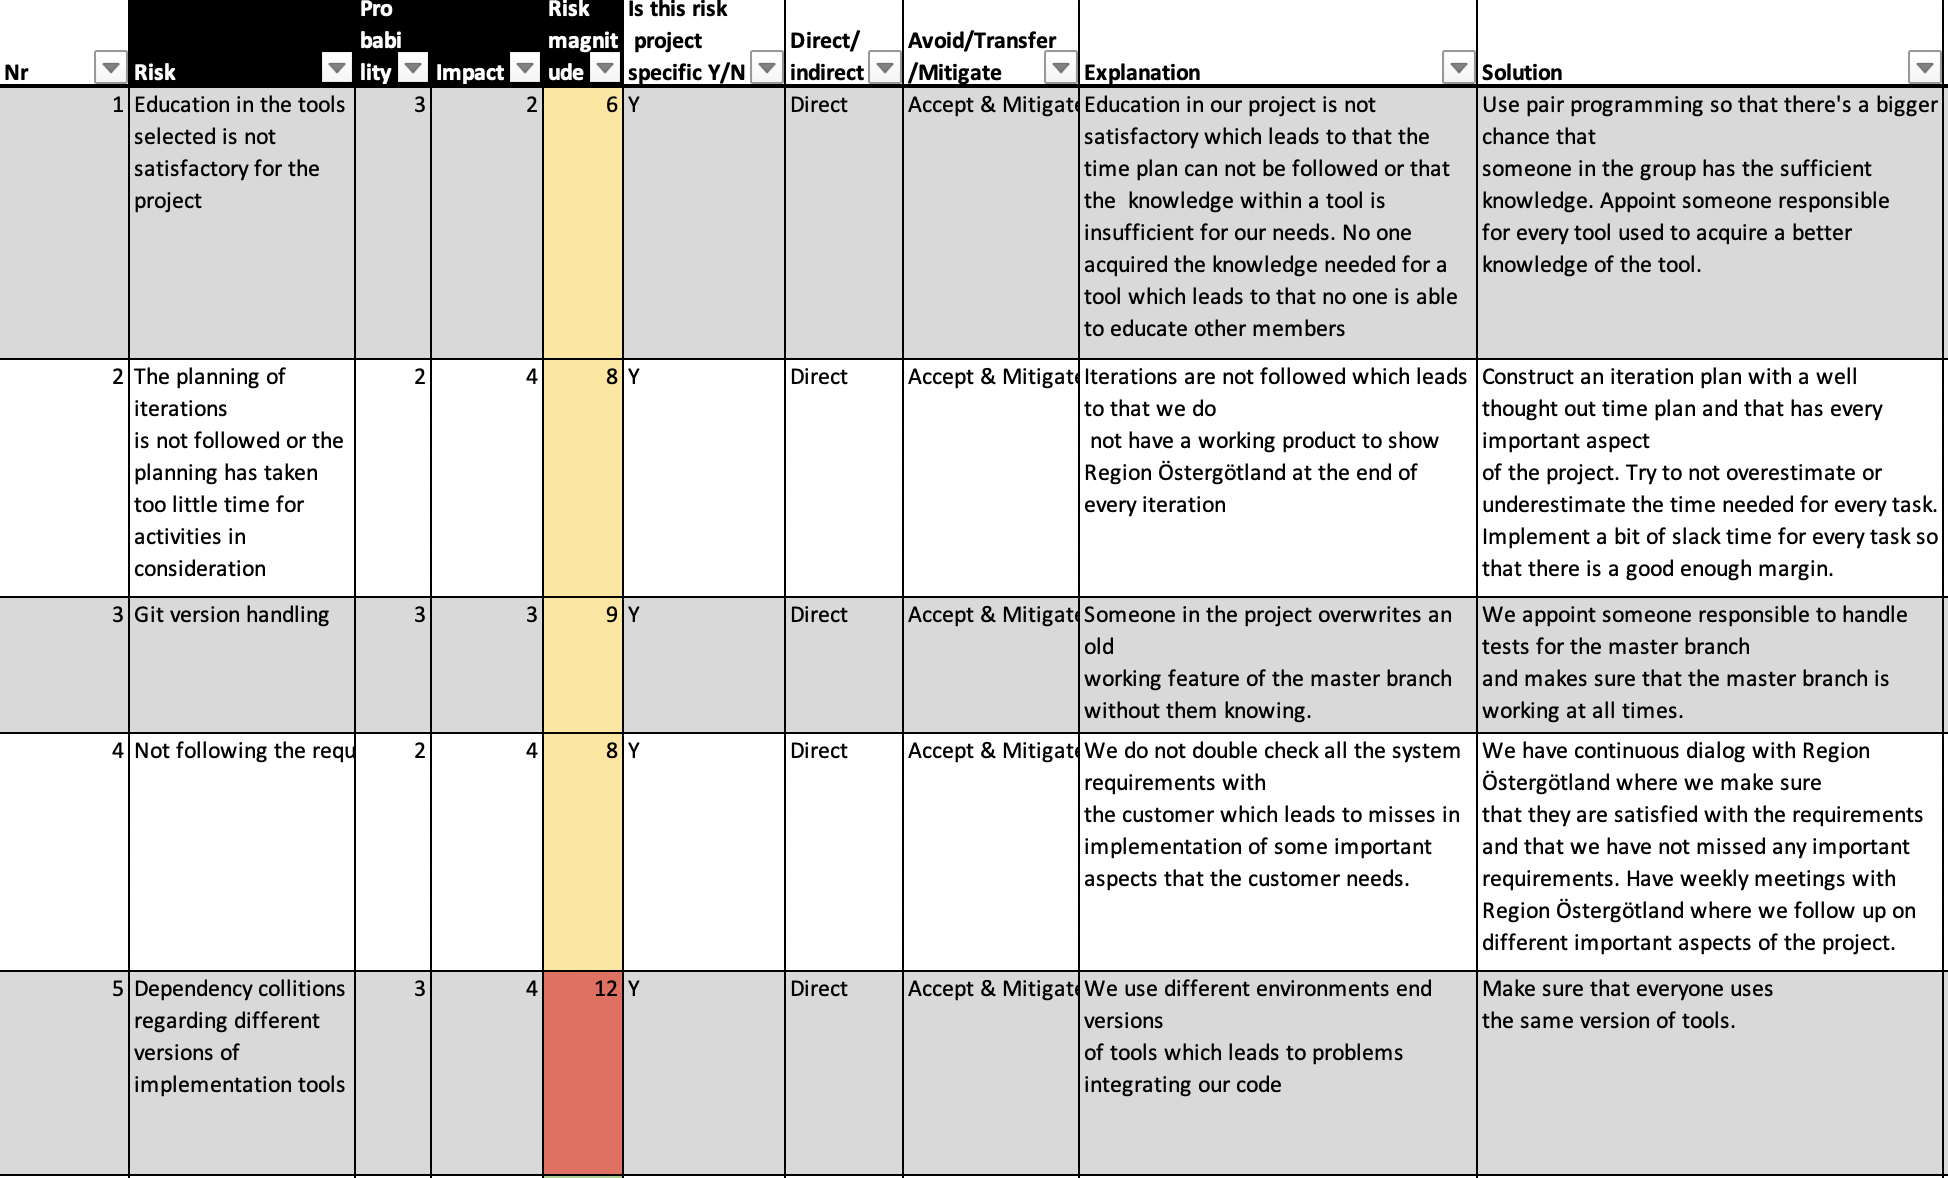
\includegraphics[width=\linewidth]{risk_analysis.jpg}}
\caption{Risks that the project is facing and how to best manage them}
\label{fig:risk_analysis}
\end{figure}
